\documentclass[border=6pt]{standalone}
\usepackage{tikz}
\usetikzlibrary{arrows.meta,calc,decorations.pathreplacing,positioning}
\begin{document}

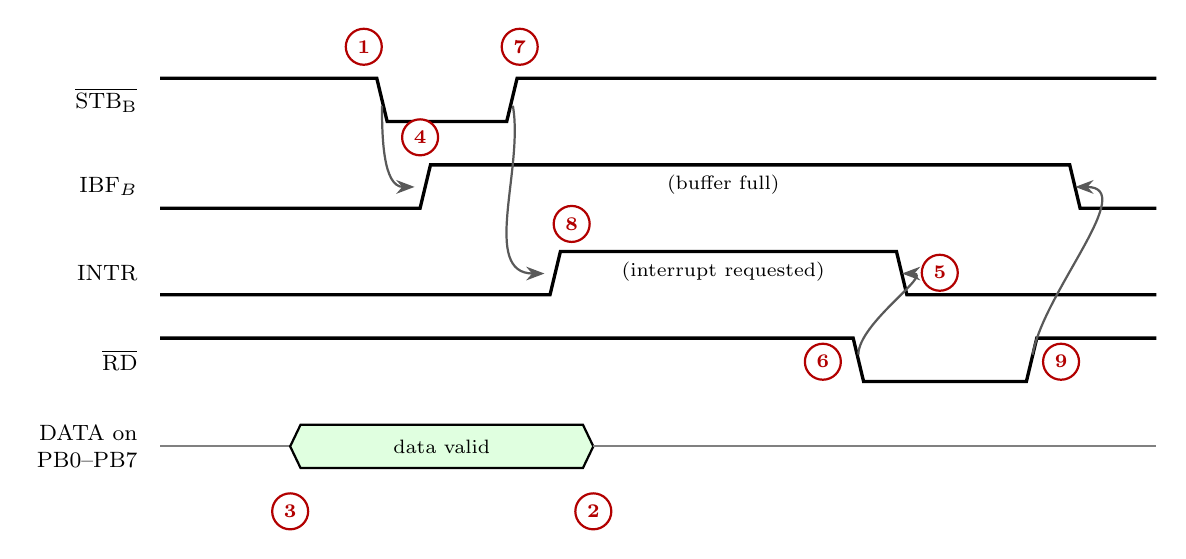
\begin{tikzpicture}[>=Stealth,font=\small,x=1.1cm,y=1cm]
% row 0 y=0
\node[anchor=east,font=\footnotesize,align=right] at (-0.15,0.275) {$\overline{\mathrm{STB_B}}$};
\draw[very thick] (0,0.55) -- (2.5,0.55) -- (2.62,0) -- (4,0) -- (4.12,0.55) -- (11.5,0.55);
% row 1 y=-1.1
\node[anchor=east,font=\footnotesize,align=right] at (-0.15,-0.825) {IBF$_B$};
\draw[very thick] (0,-1.1) -- (3,-1.1) -- (3.12,-0.55) -- (10.5,-0.55) -- (10.62,-1.1) -- (11.5,-1.1);
% row 2 y=-2.2
\node[anchor=east,font=\footnotesize,align=right] at (-0.15,-1.925) {INTR};
\draw[very thick] (0,-2.2) -- (4.5,-2.2) -- (4.62,-1.65) -- (8.5,-1.65) -- (8.62,-2.2) -- (11.5,-2.2);
% row 3 y=-3.3
\node[anchor=east,font=\footnotesize,align=right] at (-0.15,-3.025) {$\overline{\mathrm{RD}}$};
\draw[very thick] (0,-2.75) -- (8,-2.75) -- (8.12,-3.3) -- (10,-3.3) -- (10.12,-2.75) -- (11.5,-2.75);
% row 4 y=-4.4
\node[anchor=east,font=\footnotesize,align=right] at (-0.15,-4.125) {DATA on\\PB0--PB7};
\draw[thick,gray] (0,-4.125) -- (1.5,-4.125);
\draw[thick,fill=green!12] (1.5,-4.125) -- (1.62,-3.85) -- (4.88,-3.85) -- (5,-4.125) -- (4.88,-4.4) -- (1.62,-4.4) -- cycle;
\node[font=\scriptsize] at (3.25,-4.125) {data valid};
\draw[thick,gray] (5,-4.125) -- (11.5,-4.125);

\tikzset{ev/.style={circle,draw=red!70!black,thick,fill=white,font=\scriptsize\bfseries,text=red!70!black,inner sep=1pt,minimum size=13pt}}
\tikzset{cz/.style={->,thick,gray!70!black,shorten >=2pt,shorten <=2pt}}
% cause -> effect (as in the printed diagram)
\draw[cz] (2.56,0.27) to[out=-90,in=180] (3.0,-0.83);
\draw[cz] (4.06,0.27) to[out=-80,in=180] (4.5,-1.93);
\draw[cz] (8.06,-3.03) to[out=90,in=0] (8.5,-1.93);
\draw[cz] (10.06,-3.03) to[out=80,in=0] (10.5,-0.83);
% event IDs at their first occurrence
\node[ev] at (1.5,-4.95) {3};
\node[ev] at (2.35,0.95) {1};
\node[ev] at (3.0,-0.2) {4};
\node[ev] at (4.15,0.95) {7};
\node[ev] at (4.75,-1.3) {8};
\node[ev] at (5.0,-4.95) {2};
\node[ev] at (7.65,-3.05) {6};
\node[ev] at (9.0,-1.92) {5};
\node[ev] at (10.4,-3.05) {9};
\node[font=\scriptsize] at (6.5,-0.8) {(buffer full)};
\node[font=\scriptsize] at (6.5,-1.9) {(interrupt requested)};

\end{tikzpicture}
\end{document}
